%\subsection{Portfolio f\"ur Evaluation Guideline und Threats to Validity Guideline (Gr\"o\ss{}e entspricht der Anzahl)}
%\begin{figure}
\begin{center}
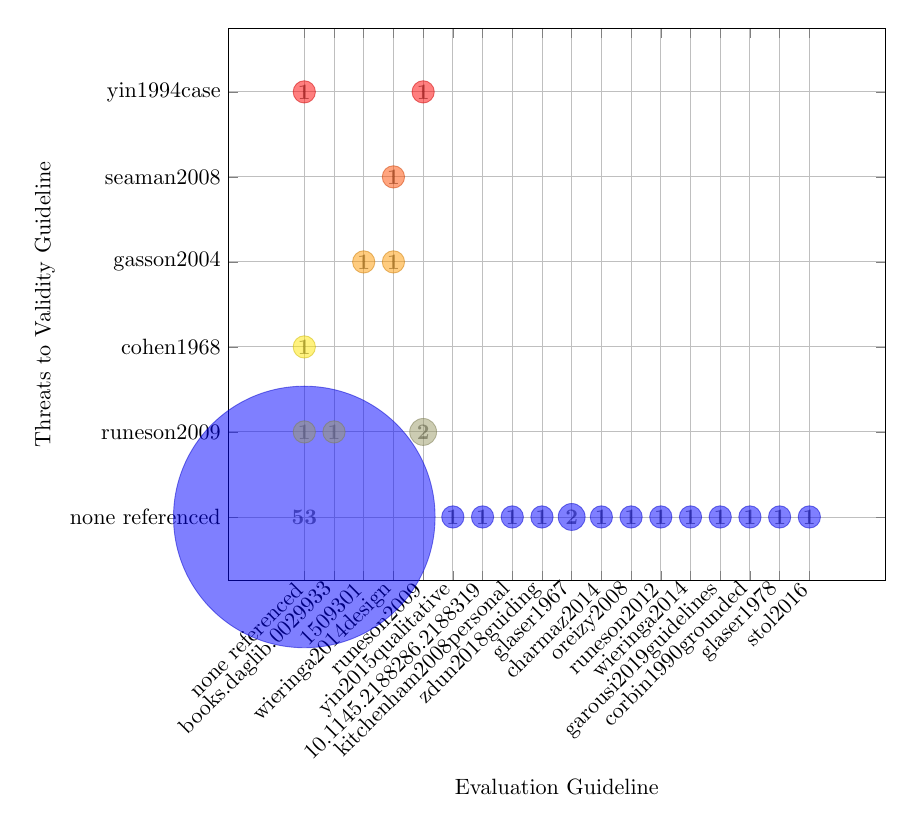
\begin{tikzpicture}[scale=.8]
\begin{axis}[scatter,
    width=.99\linewidth,
    cycle multi list=Spectral,
    every axis plot/.append style={draw, fill, fill opacity=0.5},
    scatter src=y,
    nodes near coords style={color=black,font=\small},
    enlargelimits=0.15,
    x tick label style={rotate=45,anchor=east},
    xtick={0,1,2,3,4,5,6,7,8,9,10,11,12,13,14,15,16,17}, xticklabels={none referenced,books.daglib.0029933,1509301,wieringa2014design,runeson2009,yin2015qualitative,10.1145.2188286.2188319,kitchenham2008personal,zdun2018guiding,glaser1967,charmaz2014,oreizy2008,runeson2012,wieringa2014,garousi2019guidelines,corbin1990grounded,glaser1978,stol2016},
    xlabel={Evaluation Guideline},
    ytick={0,1,2,3,4,5}, yticklabels={none referenced,runeson2009,cohen1968,gasson2004,seaman2008,yin1994case},
    ylabel={Threats to Validity Guideline},
    grid=both
]

\addplot[mark size=59.065,opacity=0.5,text=black] coordinates { (0,0) } node[text=black,font=\bfseries] {53};
\addplot[mark size=5.039,opacity=0.5,text=black] coordinates { (0,1) } node[text=black,font=\bfseries] {1};
\addplot[mark size=5.039,opacity=0.5,text=black] coordinates { (0,2) } node[text=black,font=\bfseries] {1};
\addplot[mark size=5.039,opacity=0.5,text=black] coordinates { (0,5) } node[text=black,font=\bfseries] {1};
\addplot[mark size=5.039,opacity=0.5,text=black] coordinates { (1,1) } node[text=black,font=\bfseries] {1};
\addplot[mark size=5.039,opacity=0.5,text=black] coordinates { (2,3) } node[text=black,font=\bfseries] {1};
\addplot[mark size=5.039,opacity=0.5,text=black] coordinates { (3,3) } node[text=black,font=\bfseries] {1};
\addplot[mark size=5.039,opacity=0.5,text=black] coordinates { (3,4) } node[text=black,font=\bfseries] {1};
\addplot[mark size=6.078,opacity=0.5,text=black] coordinates { (4,1) } node[text=black,font=\bfseries] {2};
\addplot[mark size=5.039,opacity=0.5,text=black] coordinates { (4,5) } node[text=black,font=\bfseries] {1};
\addplot[mark size=5.039,opacity=0.5,text=black] coordinates { (5,0) } node[text=black,font=\bfseries] {1};
\addplot[mark size=5.039,opacity=0.5,text=black] coordinates { (6,0) } node[text=black,font=\bfseries] {1};
\addplot[mark size=5.039,opacity=0.5,text=black] coordinates { (7,0) } node[text=black,font=\bfseries] {1};
\addplot[mark size=5.039,opacity=0.5,text=black] coordinates { (8,0) } node[text=black,font=\bfseries] {1};
\addplot[mark size=6.078,opacity=0.5,text=black] coordinates { (9,0) } node[text=black,font=\bfseries] {2};
\addplot[mark size=5.039,opacity=0.5,text=black] coordinates { (10,0) } node[text=black,font=\bfseries] {1};
\addplot[mark size=5.039,opacity=0.5,text=black] coordinates { (11,0) } node[text=black,font=\bfseries] {1};
\addplot[mark size=5.039,opacity=0.5,text=black] coordinates { (12,0) } node[text=black,font=\bfseries] {1};
\addplot[mark size=5.039,opacity=0.5,text=black] coordinates { (13,0) } node[text=black,font=\bfseries] {1};
\addplot[mark size=5.039,opacity=0.5,text=black] coordinates { (14,0) } node[text=black,font=\bfseries] {1};
\addplot[mark size=5.039,opacity=0.5,text=black] coordinates { (15,0) } node[text=black,font=\bfseries] {1};
\addplot[mark size=5.039,opacity=0.5,text=black] coordinates { (16,0) } node[text=black,font=\bfseries] {1};
\addplot[mark size=5.039,opacity=0.5,text=black] coordinates { (17,0) } node[text=black,font=\bfseries] {1};


\end{axis}
\end{tikzpicture}
\end{center}
%\caption{Portfolio f\"ur Evaluation Guideline und Threats to Validity Guideline (Gr\"o\ss{}e entspricht der Anzahl)}\label{fig:port_evaluationguideline_threatstovalidityguideline}
%\end{figure}

